\chapter{Developer documentation}
\label{ch:impl}

\section{Building the code}

There are currently two ways of building the code on Windows OS either with Visual Studio and using \textbf{vcpkg} as the package manager or with \textbf{MinGW} and manually building the packages (which I have deprecated but it's possible and I have put it in a separate branch).

First the following steps must be fulfilled to start developing (on windows):

\begin{itemize}
	\item Install \textbf{vcpkg} and add it to your path.
	\item Run the integrate install command so Visual Studio can detect it.
	\item Install CMake.
\end{itemize}

\subsection{Building with CMake}

To make it easier to download the required packages, a powershell script \texttt{install\_dependencies.ps1} is provided with the code which installs all the required dependencies.

Then the project can be built with CMake either by running \texttt{build\_for\_vs.ps1} script or by doing the following in the shell:
\lstset{caption={Building with CMake}, label=src:sh}
\begin{lstlisting}[language=bash]
mkdir build
cd build
cmake .. -G "Visual Studio 17 2022" -A x64 -DCMAKE_TOOLCHAIN_FILE=%PATH_TO_VCPKG%/scripts/buildsystems/vcpkg.cmake
\end{lstlisting}

You can replace generator with your compiler of liking, MinGW, for instance (if you have the packages installed). Replace the tool chain file path to your vcpkg path. 

CMake was chosen because of its cross-platform support. If, for instance, you want to build on linux and have the required packages then you can build using the same CMake file, in which case it will generate a Makefile instead of the VS solution.

\section{Design and the rendering pipeline}
This sections describes how the components fit together and in what order the things are rendered before proceeding to explain all steps in detail.

\subsection{The OpenGL Rendering Pipeline}
\begin{figure}[H]
    \centering
    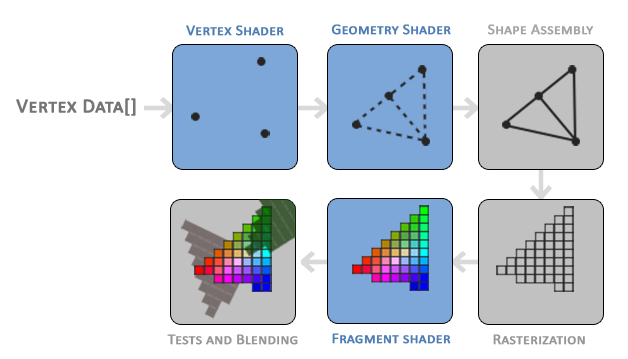
\includegraphics[width=0.75\textwidth]{images/opengl_pipeline.png}
    \caption{The OpenGL Pipeline} \cite{learnopengl}
    \label{fig:opengl_pipeline}
\end{figure}

First let's look at the OpenGL rendering pipeline in Figure~\ref{fig:opengl_pipeline}. The only procedures that we are concerned with at the moment are Vertex and Fragment shaders. Geometry shaders will be described at a later stage when they are needed.

\begin{definition}{Shaders}
	Shaders are programs that run on the GPU, there are various ways to send data to shaders. In the code, I mainly send data through vertex buffers or through uniforms. 
\end{definition}

Without going into too much depth, vertex shaders transform vertices from local space to normalized device coordinates and fragment shaders are used for choosing the colors (as depicted in the picture above).

\subsection{Vertex Shader Convention}
The code snippet below describes how a typical vertex shader looks like in the code:
\lstset{caption={Vertex shader convention}, label=src:vertex_convention}
\begin{lstlisting}[language=C]
layout (location = 0) in vec3 aPos;

uniform mat4 proj;
uniform mat4 view;
uniform mat4 model;

void main() {
	gl_Position = proj * view * model * vec4(aPos, 1.0);
}

\end{lstlisting}

In this document, I will be representing the projection matrix as $\mathbf{P}$, view as $\mathbf{V}$, and model as $\mathbf{M}$. In some vertex shaders there is also a local transformation matrix because I sometimes like to dissect the model matrix into two matrices the model and the local matrix, the former puts the object into the world space and the local transformation is responsible for any rotation or scaling.

\subsection{Shader loader}
To make it easier to load, compile and use shaders the engine comes with a Shader loading
class. The design of the shader loader/manager is inspired by the one on LearnOpenGL \cite{learnopengl}. This class is responsible for allocating and destructing the shaders. A different class is also defined specifically for loading Compute shaders which will be described later. However, the interface for using and setting the uniform variables is identical for both classes.

Uniform variables can easily be set using this shader class, as illustrated in the code snippet below (all such functions can be found in the header file):
\lstset{caption={Shader class usage example}, label=src:shader_usage}
\begin{lstlisting}[language=C++]
Shader myShader {"vertexSource.glsl", "fragmentSource.glsl"};
myShader.use();
myShader.setVec3("cameraPos", glm::vec3(0.0f));
\end{lstlisting}

\subsection{Mesh handling}
\label{subsec:mesh_handling}
In OpenGL the mesh data must be transferred to a \textbf{VBO (Vertex Buffer Object)} first and then the \textbf{VBO} must be bound to a \textbf{VAO (Vertex Array Object)}, instructions for how to parse the data in \textbf{VBO} must also be explicitly defined and optionally a drawing order of vertices can also be defined in a \textbf{EBO (Element Buffer Object)}. To make this simpler a \textbf{Mesh} class comes with the engine. This is also inspired by an implementation on LearnOpenGL \cite{learnopengl}. The figure below gives a rough UML of how the mesh class is structured.

\begin{figure}[H]
    \centering
    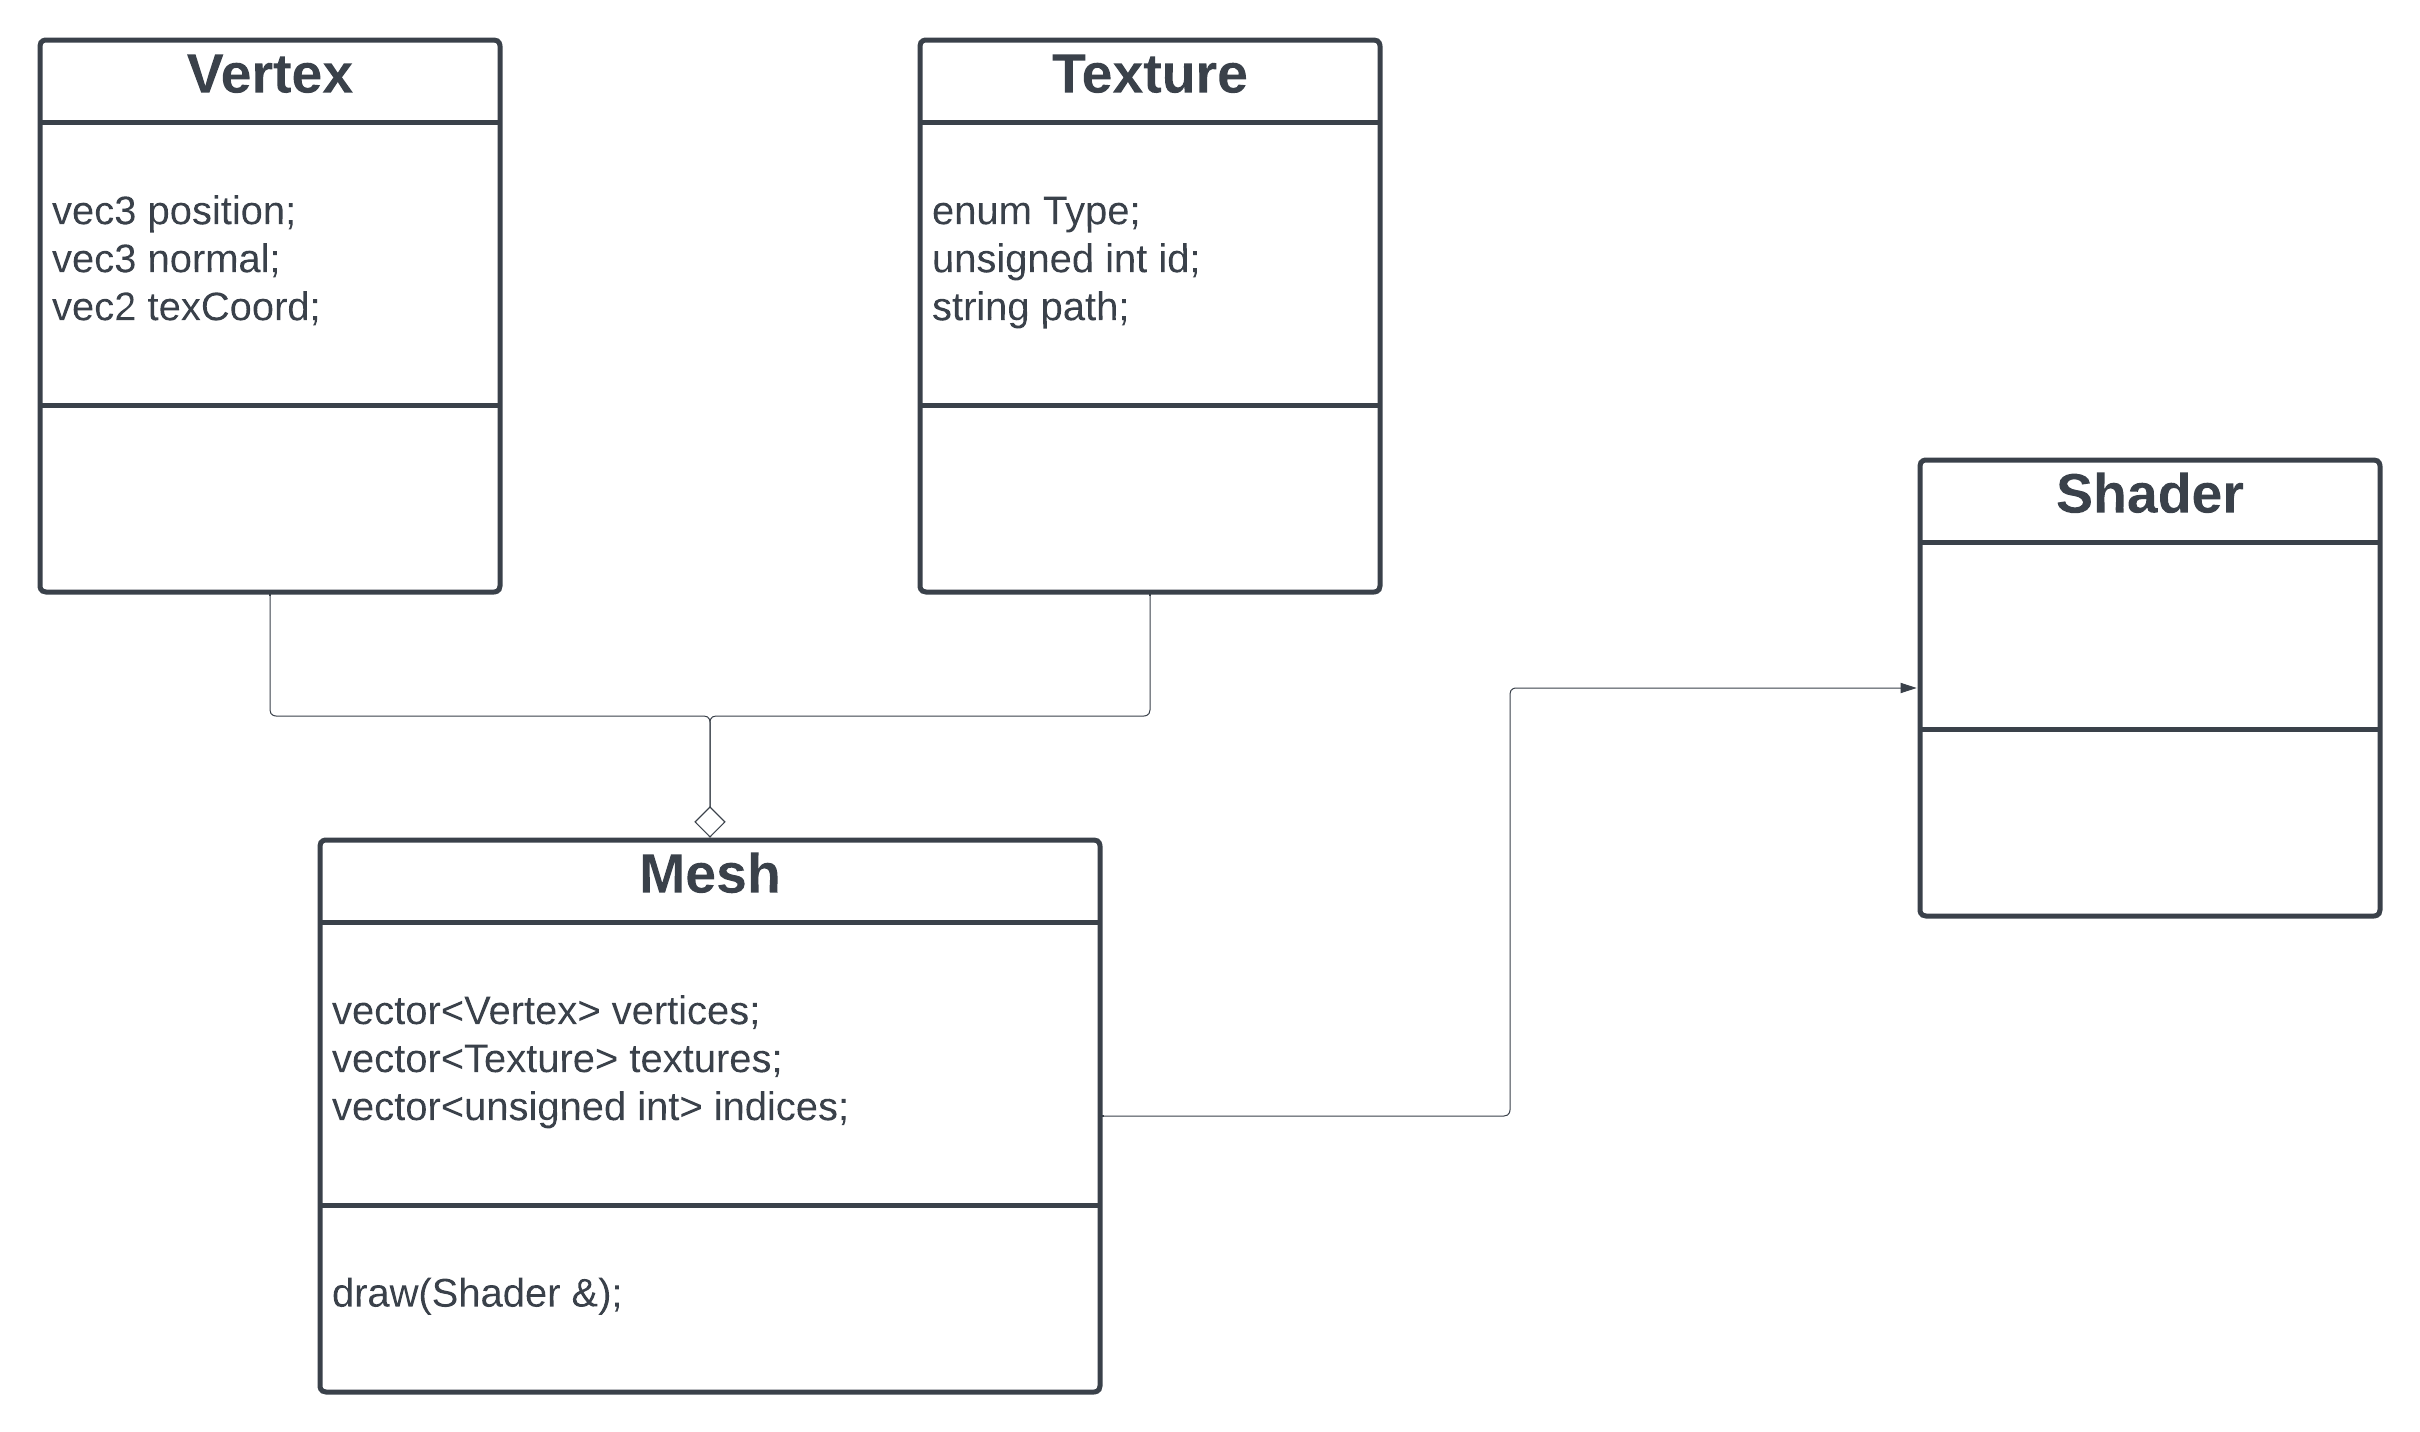
\includegraphics[width=0.75\textwidth]{images/mesh_uml.png}
    \caption{Mesh Class} \cite{learnopengl}
    \label{fig:mesh_uml}
\end{figure}

Meshes for 3d can be generated easily using a mapping $f (u, v)\rightarrow 
\langle x, y, z \rangle$. Some simple examples are given in \texttt{funcs.h} and \texttt{funcs.cpp}. For instance, a sphere can be generated using the function: $f (\theta, \phi) \rightarrow \langle \cos\theta\cos\phi, \sin\phi, \sin\theta\cos\phi \rangle$, where $\theta \in [0, 2\pi], \phi \in [-\frac{\pi}{2}, \frac{\pi}{2}]$. The normal vector for a sphere $\hat{n}$ is, of course, the same as $f (\theta, \phi)$. An implementation for generating the mesh of a torus is also given; a simple version of which can be derived by taking the parametric equation of a circle and translating it along, say, the x axis by $r\prime$: $C (\theta) = \langle r\cos\theta+r\prime, r\sin\theta, 0 \rangle$. If $\mathbf{R_y (\phi)}$ is the rotation around y axis then the torus is $f (\theta, \phi) = \mathbf{R_y( \phi)}C( \theta)$ where $\theta, \phi \in [0, 2\pi]$.


\subsection{Model loading}
The first implementation was done with a custom object file loader, however, it is infeasible to write a complete model loader that triangulates the vertices, supports multiple formats, and pares the texture files accurately. So, the decision to use \textbf{assimp} was made. The \textbf{Model} class is basically a wrapper around \textbf{assimp} functionality. This implementation was also motivated by the one provided on LearnOpenGL \cite{learnopengl}, however, contrary to that implementation this one is more optimized and handles the loading of materials more accurately.

The figure below can be used as a reference for understanding the code in the Model class.
\begin{figure}[H]
    \centering
    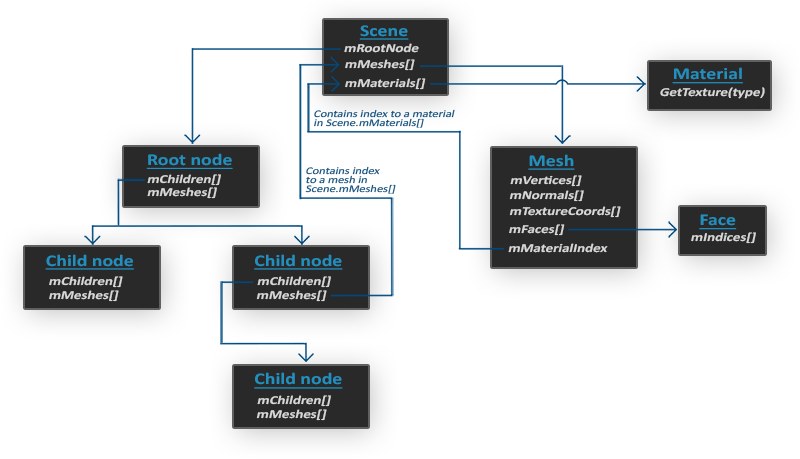
\includegraphics[width=0.75\textwidth]{images/assimp_structure.png}
    \caption{Assimp Structure} \cite{learnopengl}
    \label{fig:assimp_structure}
\end{figure}

A model can be thought of as a collection of meshes, so the rough UML diagram of the class below should make sense:
\begin{figure}[H]
    \centering
    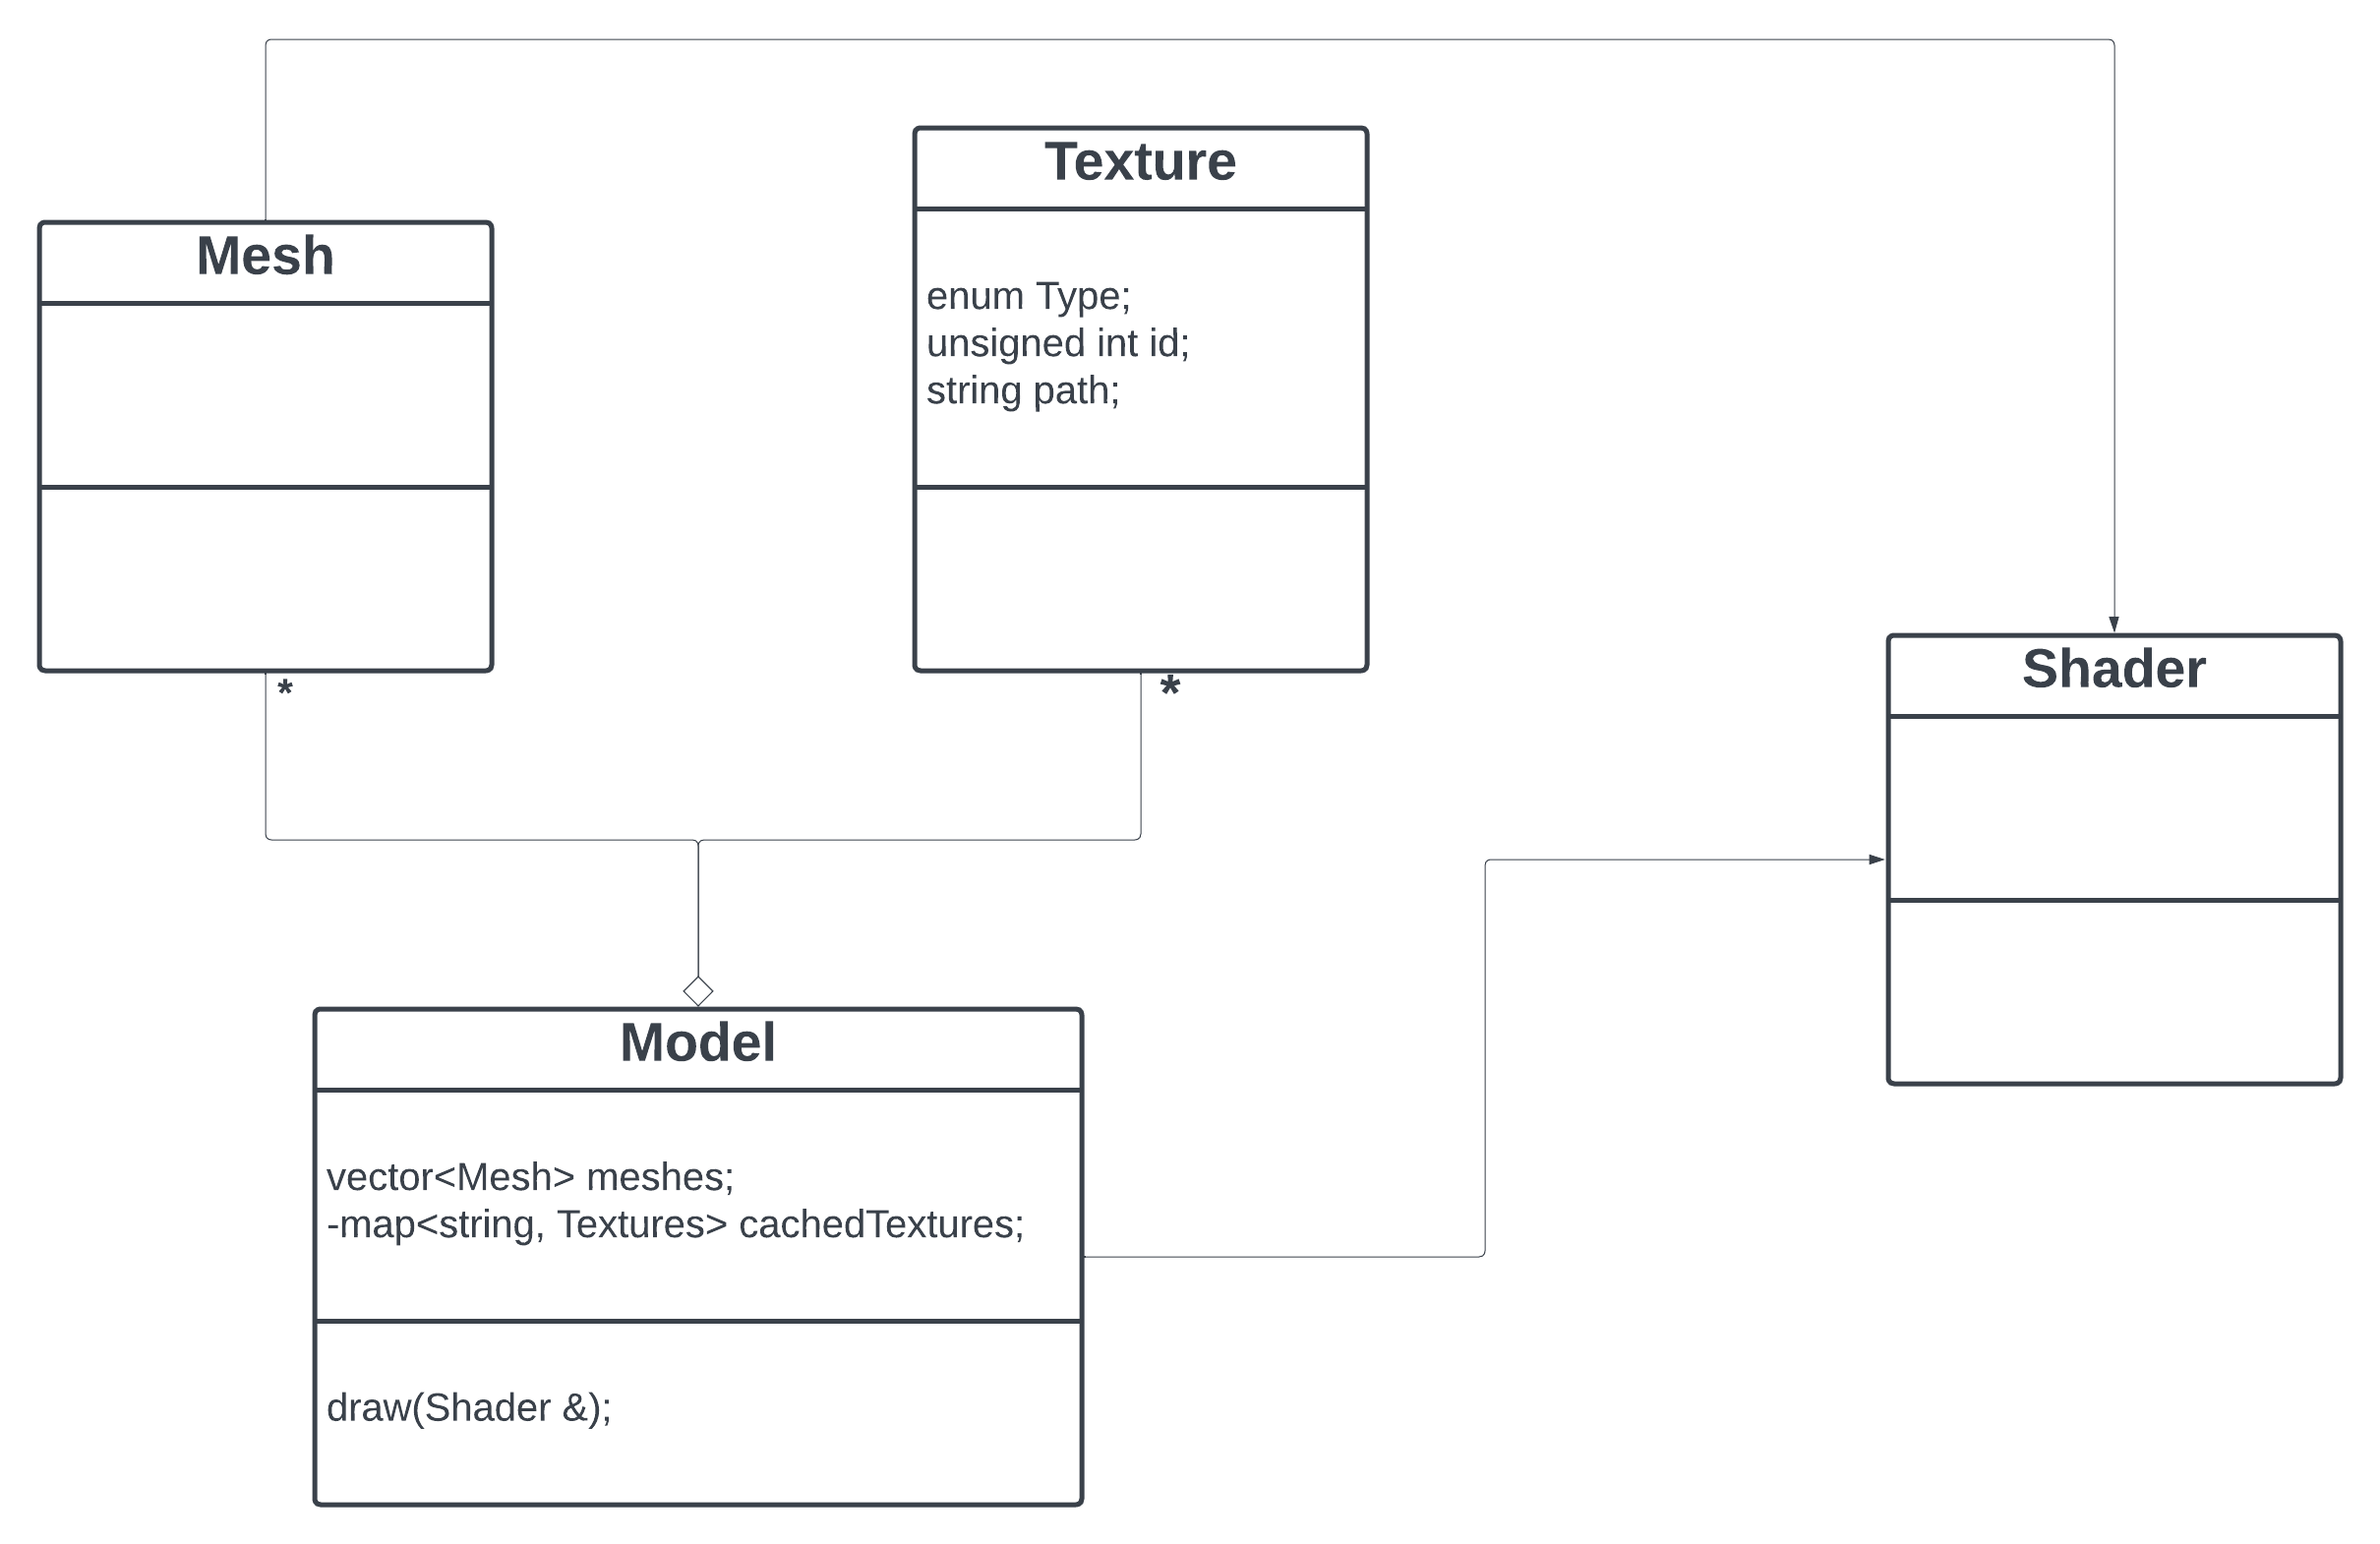
\includegraphics[width=0.5\textwidth]{images/model_uml.png}
    \caption{Model class UML}
    \label{fig:model_uml}
\end{figure}

Since models can have multiple diffuse and specular textures, they must be defined in the shaders in following convention. Diffuse textures must follow the following naming \textbf{texture\_diffuse[1..]}, specular textures must be named as \textbf{texture\_specular[1..]}.


\subsection{\texttt{Camera} class and the camera transform}

\begin{figure}[H]
    \centering
    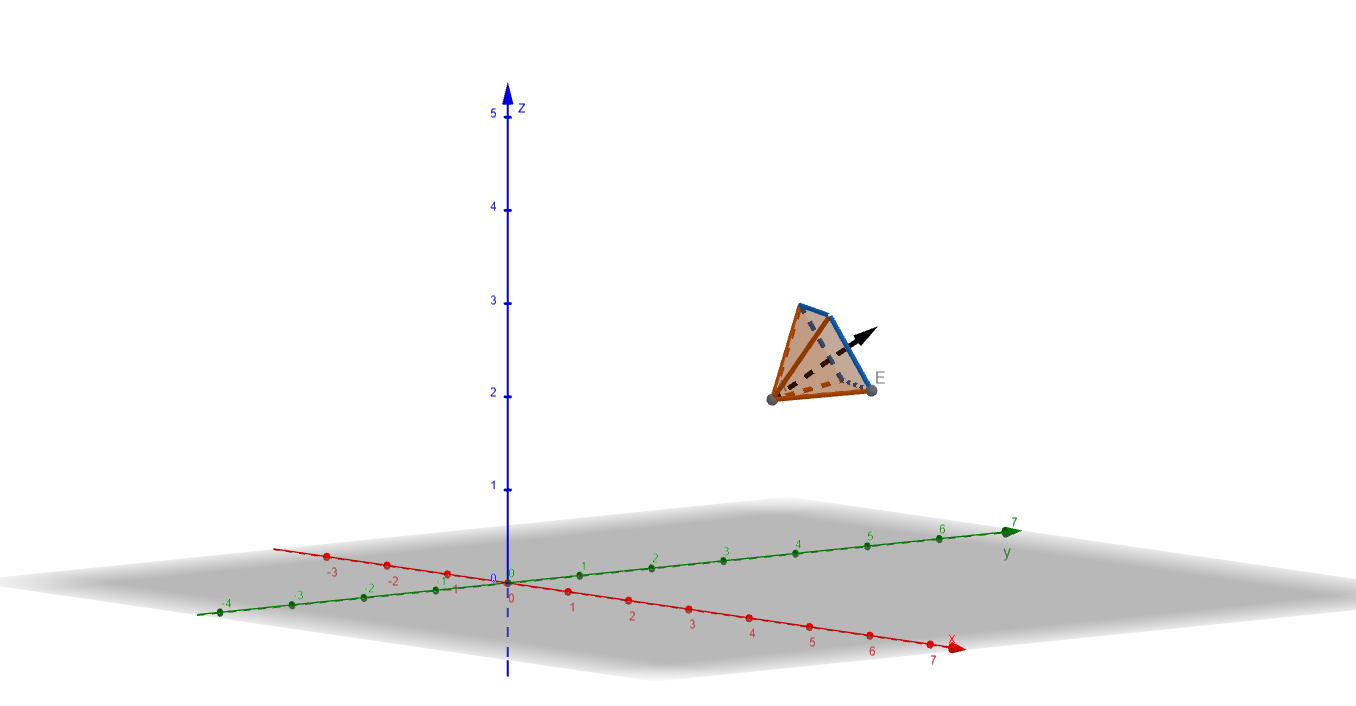
\includegraphics[width=0.75\textwidth]{images/camera_eg2.png}
    \caption{Simple Camera example}
    \label{fig:camera_eg}
\end{figure}

The camera can be imagined as a vector in the figure above. It sits at a point $\mathbf{p}$ looking in direction {$\mathbf{\hat{d}}$}. Contrary to some common implementations, which store a lookAt variable to store what point the camera is looking at, I only store the direction which can be dissected into two components: pitch (rotation around the $x-axis$), represented as $\phi$, and yaw (rotation around the $y-axis$) which is represented as $\theta$. Similar to what was done in the meshes section~\ref{subsec:mesh_handling}, it can be observed that these define a spherical coordinate system and we can get $\mathbf{\hat{d}}$ as follows: \begin{equation}\mathbf{\hat{d}} = \langle \cos\theta\cos\phi, \sin\phi, \sin\theta\cos\phi \rangle\end{equation}

However, the pitch is constrained to avoid distortions so, $\phi \in [-\frac{\pi}{4}, \frac{\pi}{4}]$. An absolute up direction vector is also defined for the camera which I will denote as $\hat{u}$ and $\hat{u}=\langle0, 1, 0\rangle$. The projection matrix works by assuming that the camera is looking in the negative $z-axis$ and is sitting at the origin. So $\mathbf{V}$ must be the matrix that puts the camera in this position. $\mathbf{V}$ must first translate the camera to the origin and then apply the inverse rotation of the current camera rotation.

If $\vec{p}$ is the position vector of the camera, then let $\mathbf{T_{-\overrightarrow{p}}}$ represent the translation matrix that translates by $-{\vec{p}}$.


The current rotation matrix of the camera can be obtained by getting the front (but flipped because the camera starts by looking in the negative $z$-axis), right, and up vectors of the camera:

\[
\hat{f} = \text{front} = -\hat{d}
\]
\[
\hat{r} = \text{right} = \hat{d} \times \hat{u}
\]
\[
\hat{a} = \text{up} = \hat{r} \times \hat{d}
\]

The rotation matrix is then:

\[
\mathbf{R} = \begin{bmatrix} 
\hat{r} & \hat{a} & \hat{f} 
\end{bmatrix}
\]

This can be imagined as where the $\hat{i}, \hat{j}, \hat{k}$ vectors land after the transformation.

We want the inverse of this matrix. Since this is an orthonormal matrix, the inverse is the transpose of the matrix:

\[
\mathbf{R^{-1}} = \mathbf{R}^T
\]

Thus, the final view matrix is:

\[
\mathbf{V} = \mathbf{R}^T \mathbf{T}_{-\mathbf{\overrightarrow{p}}}
\]


The \texttt{Camera} class in the code provides the above functionalities, and the view matrix can be easily obtained by calling the \texttt{camera.getView()} method.

\subsection{Audio Manager}

The engine includes an audio manager capable of playing 2D sounds. Currently, there is no implementation available for 3D audio playback. This component serves as a wrapper around the functionality provided by \textbf{OpenAL}. Audio files are loaded using \textbf{libsndfile}, and the engine currently supports only the \textbf{WAV} format.

The following code snippet demonstrates a basic usage example:

\lstset{caption={Audio Manager example}, label=src:audio_manager}
\begin{lstlisting}[language={C++}]
#include <audio_manager.h>
#include <iostream>

int main() 
{
    AudioManager audioMgr;
    audioMgr.play2d("soundfile.wav", /*loop*/ false);
    std::cin.get(); // prevent exiting
}
\end{lstlisting}


% TO DO: add text renderer, sprite renderer, explain homogenous coords if time permits.

\subsection{OpenGL Frame Buffer Objects and the \texttt{FrameBuffer} Class}

OpenGL provides Frame Buffer Objects (FBOs), which can be thought of as off-screen rendering targets—similar to virtual canvases or pseudo-windows that you can draw on. Instead of rendering directly to the screen, FBOs allow rendering to a texture or render buffer. This is particularly useful for post-processing effects, shadow mapping, and deferred rendering techniques.

The \texttt{FrameBuffer} class in the engine serves as a wrapper around OpenGL’s FBO functionality, simplifying the creation, configuration, usage, and memory management of frame buffer objects. It provides functionality to bind the FBO, with the option to clear it upon binding.

For simplicity, this implementation constructs the FBO using textures (rather than \textbf{Renderbuffer Objects}), as most parts of the engine require the ability to read from the framebuffer. A depth buffer is also included. These design choices can be modified in the future to support more flexible configurations.

A simple example is provided below:

\lstset{caption={Frame Buffer example}, label=src:frame_buffer}
\begin{lstlisting}[language={C++}]
#include <framebuffer.h>
#include <iostream>

int main() 
{
    // Ensure OpenGL context is active before using the FrameBuffer
    FrameBuffer frameBuffer;
    frameBuffer.bind();

    // All OpenGL draw calls will now render to the frame buffer
    // ...

    frameBuffer.unBind();

    // Access the color and depth texture IDs if needed
    GLuint colorTex = frameBuffer.textureId;
    GLuint depthTex = frameBuffer.depthTextureId;

    // Or, draw the FBO's content directly to the screen
    frameBuffer.draw(); 
}
\end{lstlisting}


\subsection{Architecture}

The UML diagram below represents a simplified architecture of the whole game and shows how the components connect to each other.

\begin{figure}[H]
    \centering
    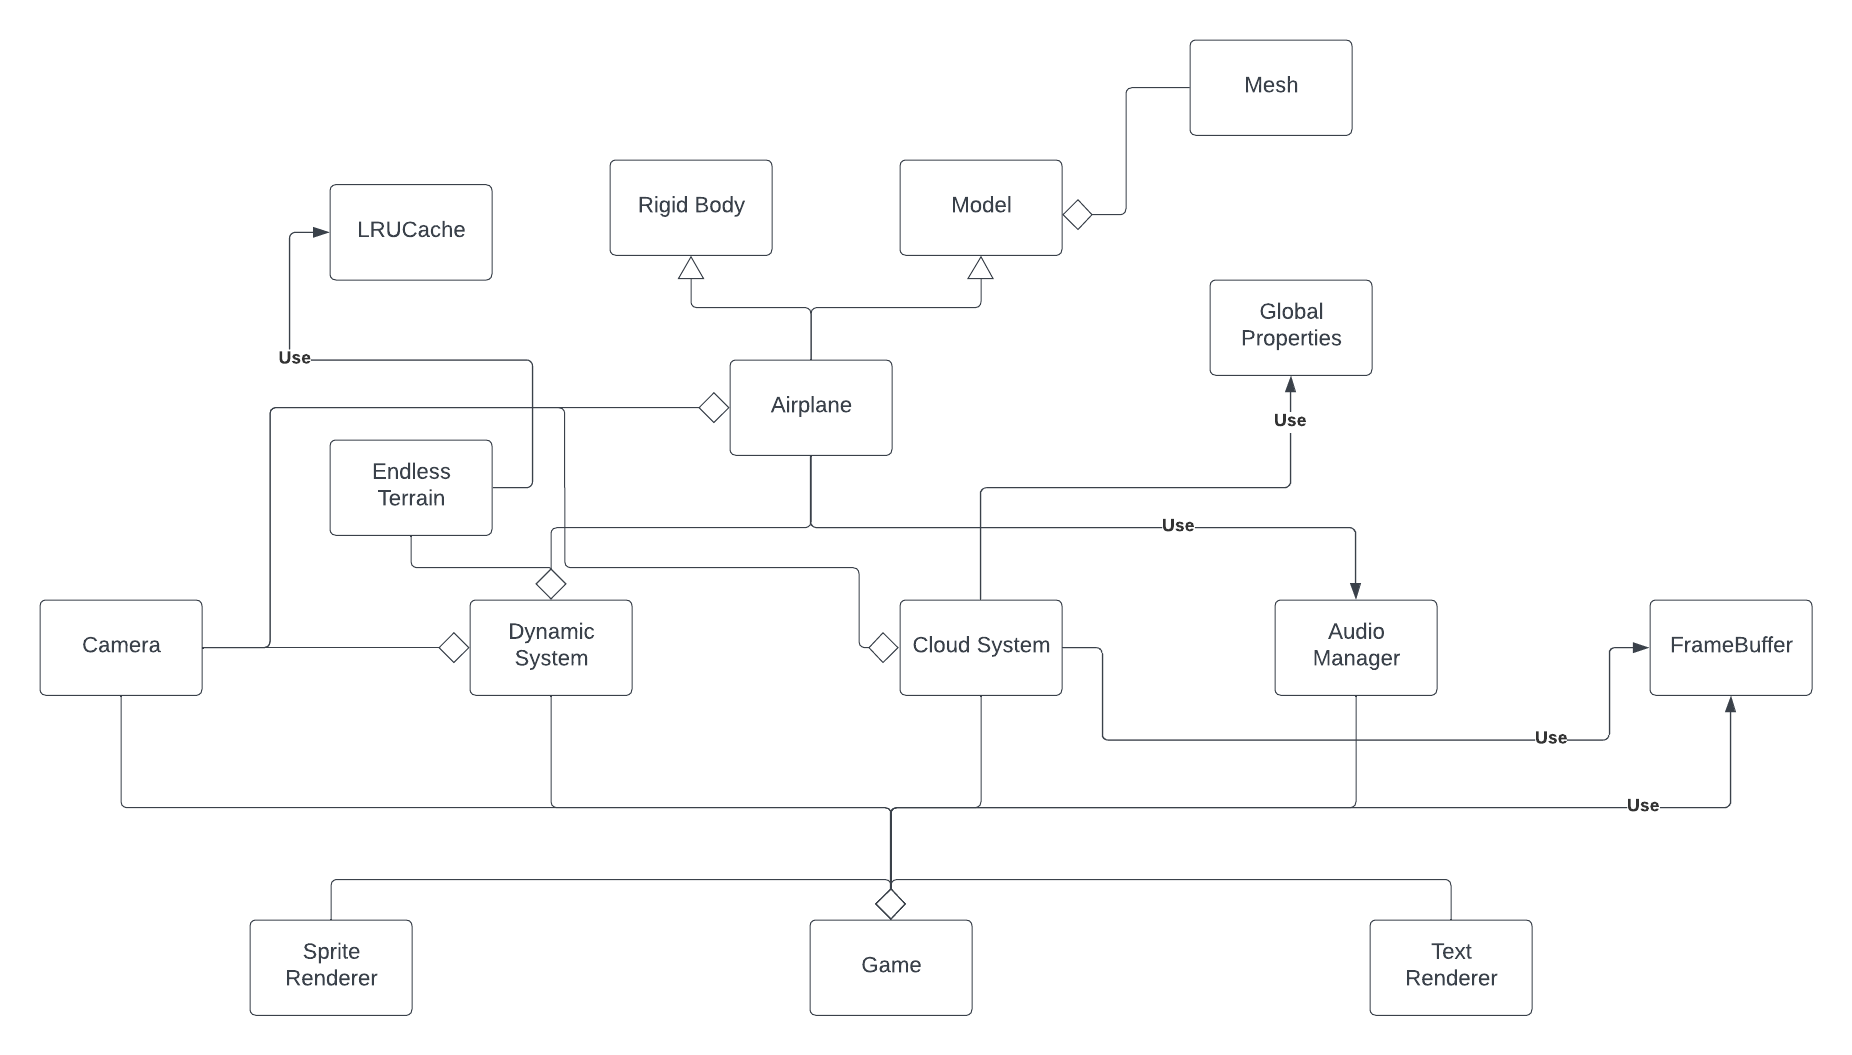
\includegraphics[width=1.0\textwidth]{images/architecture.png}
    \caption{Architecture}
    \label{fig:architecture}
\end{figure}


The main components i.e endless terrain, cloud system, rigid body, and airplane are explained the following sections.

\section{Procedural Terrain}

\subsection{Generating a chunk}

\begin{definition}[Chunk]
A \textit{chunk} refers to a rectangular mesh of predefined size, where each vertex contains height and normal vector information. Chunks serve as the basic building blocks for terrain generation and rendering.
\end{definition}

In most implementations where non-repetitive chunks are required, noise algorithms are commonly used. The algorithm I have chosen is \textbf{Perlin Noise} \cite{perlin2002improving}, which is implemented in \texttt{perlin.cpp}. Assuming, for now that we have some sort of a Perlin noise implementation available, a chunk that only has height data may be generated as simply as the following pseudo code shows:

\lstset{caption={Chunk generation}, label=src:frame_buffer}
\begin{lstlisting}[language=Python]
def generateChunkData(size, scale):
	chunkData = ChunkData(size, size)
	for i in range(size):
		for j in range(size):
			x = j * scale
			y = i * scale
			chunkData.height[i, j] = perlin(x, y)
	return chunkData
\end{lstlisting}

Next, we will explore how to extend this basic chunk with additional data such as normals and how to tile these chunks together for a continuous terrain. We will also dive into techniques such as Level of Detail (LOD) and early culling, which help improve performance and rendering efficiency in large terrains. First, let’s simplify Perlin Noise and look at how to calculate normals for our chunk data.


\subsection{Perlin Noise}

This section does not aim to provide a detailed theoretical explanation of the Perlin Noise algorithm. For a formal treatment, the reader is encouraged to refer to the original paper by Ken Perlin \cite{perlin2002improving}. For a more intuitive and visual explanation, see the video referenced in \cite{perlin_video}. 

Perlin Noise is a type of gradient noise that aims at generating smooth noise. If we, for instance, take a look at white noise where each pixel can be thought of as having a uniform probability of having a value between 0 and 1. The generated map as illustrated in Figure~\ref{fig:white_noise} looks completely random and this would never work as a height map as the height of a terrain is continuous.

\begin{figure}[H]
    \centering
    \begin{minipage}[t]{0.45\textwidth}
        \centering
        
\includegraphics[width=\textwidth]{images/white_noise.png}
        \caption{White Noise}
        \label{fig:white_noise}
    \end{minipage}
    \hfill
    \begin{minipage}[t]{0.45\textwidth}
        \centering
        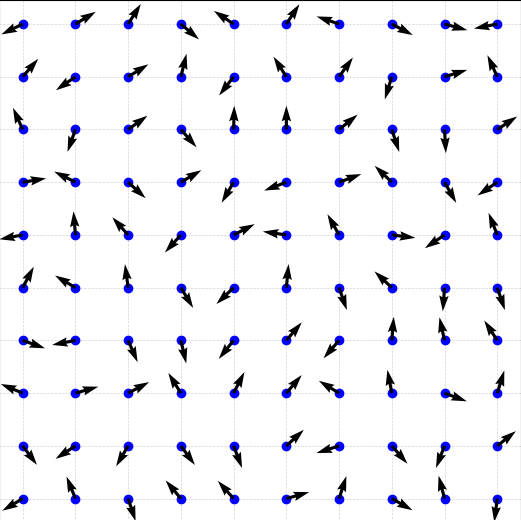
\includegraphics[width=\textwidth]{images/perlin_grid.png}
        \caption{Perlin Grid}
        \label{fig:perlin_grid}
    \end{minipage}
\end{figure}


Before looking into how Perlin noise works, let's define the \texttt{lerp} function.
\begin{definition}[\texttt{lerp}]
	Lerp is defined as :
	\[
		\texttt{lerp}(a, b, p) = a + p(b - a)
	\]
	% lerp(a, b, p) = $a + p(b-a)$
\end{definition}

% Perlin noise works by dividing a plane into a grid that has a random gradient vector assigned at each vertex as shown in Figure~\ref{fig:perlin_grid}. Let's just look at one box and call the point on the top left as $P_{tl}$ and vector associated with as $\vec{v_{tl}}$, we will label other points as $P_{tr}$, $P_{bl}$, $P_{br}$. If we take a point $U$ inside this box with coordinates ($U_x$, $U_y$), and ($u$, $v$) representing the fractional parts of ($U_x$, $U_y$) then the noise function as this point is evaluated as follows:\\
% Let $D_{tl}$ $=$ $P_{tl} - U$, $D_{tr}$, $D_{bl}$, $D_{br}$ are defined similarly. And Let $G_{tl} = \langle V_{tl}, D_{tl} \rangle$, $G_{tr}$, $G_{bl}$, $G_{br}$ are defined similarly.\\
% A step function $g(t)=6t^t-15t^4+10t^3$ is used for smoothing the values of $(u, v)$ and the noise is evaluated as 
% \begin{center}
% 	$noise(U_x, U_y)$ = \texttt{lerp}(\texttt{lerp}($G_{tl}$, $G_{tr}$, $g(u)$), \texttt{lerp}($G_{bl}$, $G_{br}$, $g(u)$), $g(v)$)
% \end{center}

Perlin noise works by dividing the plane into a grid, assigning a random gradient vector at each vertex, as shown in Figure~\ref{fig:perlin_grid}. Consider a single grid cell, and label the corners as follows:
\begin{itemize}
\item{Top-left: $P_{tl}$ with gradient $\vec{v}_{tl}$}
\item{Top-right: $P_{tr}$ with gradient $\vec{v}_{tr}$}
\item{Bottom-left: $P_{bl}$ with gradient $\vec{v}_{bl}$}
\item{Bottom-right: $P_{br}$ with gradient $\vec{v}_{br}$}
\end{itemize}

Let $U = (U_x, U_y)$ be a point inside the cell, and let $(u, v)$ be the fractional parts of $(U_x, U_y)$ relative to the cell.

Define direction vectors from each corner to $U$:
\[
\vec{d_{tl}} = U - P_{tl}, \quad \vec{d_{tr}} = U - P_{tr}, \quad \vec{d_{bl}} = U - P_{bl}, \quad \vec{d_{br}} = U - P_{br}
\]

Next, compute the dot products:
\[
G_{tl} = \langle \vec{v}_{tl}, \vec{d_{tl}} \rangle, \quad G_{tr} = \langle \vec{v}_{tr}, \vec{d_{tr}} \rangle, \quad G_{bl} = \langle \vec{v}_{bl}, \vec{d_{bl}} \rangle, \quad G_{br} = \langle \vec{v}_{br}, \vec{d_{br}} \rangle
\]

A smoothing function is used to interpolate values:
\[
g(t) = 6t^5 - 15t^4 + 10t^3
\]

Finally, the noise value at point $U$ is computed using bilinear interpolation:
\[
\texttt{noise}(U_x, U_y) = \texttt{lerp}(\texttt{lerp}(G_{tl}, G_{tr}, g(u)), \texttt{lerp}(G_{bl}, G_{br}, g(u)), g(v))
\]


\subsection{Equations, formulas}

Duis suscipit ipsum nec urna blandit, $2 + 2 = 4$ pellentesque vehicula quam fringilla. Vivamus euismod, lectus sit amet euismod viverra, dolor metus consequat sapien, ut hendrerit nisl nulla id nisi. Nam in leo eu quam sollicitudin semper a quis velit.

$$a^2 + b^2 = c^2$$

Phasellus mollis, elit sed convallis feugiat, dolor quam dapibus nibh, suscipit consectetur lacus risus quis sem. Vivamus scelerisque porta odio, vitae euismod dolor accumsan ut.

In mathematica, identitatem Euleri (equation est scriptor vti etiam notum) sit aequalitatem Equation~\ref{eq:euler}:
\begin{equation}\label{eq:euler}
e^{i \times \pi} + 1 = 0
\end{equation}

Vestibulum ante ipsum primis in faucibus orci luctus et ultrices posuere cubilia curae; Nullam pulvinar purus at pharetra elementum.
Aequationes adsignans aequationis signum:
\begin{align}
	A & = \frac{\pi r^2}{2} \\
	& = \frac{1}{2} \pi r^2
\end{align}

Proin tempor risus a efficitur condimentum. Cras lobortis ligula non sollicitudin euismod. Fusce non pellentesque nibh, non elementum tellus.
Omissa numeratione aliquarum aequationum:
\begin{align}
	f(u) & =\sum_{j=1}^{n} x_jf(u_j) \nonumber \\
	& =\sum_{j=1}^{n} x_j \sum_{i=1}^{m} a_{ij}v_i \nonumber \\
	& =\sum_{j=1}^{n} \sum_{i=1}^{m} a_{ij}x_jv_i
\end{align}

\section{Source code samples}

Nulla sodales purus id mi consequat, eu venenatis odio pharetra. Cras a arcu quam. Suspendisse augue risus, pulvinar a turpis et, commodo aliquet turpis. Nulla aliquam scelerisque mi eget pharetra. Mauris sed posuere elit, ac lobortis metus. Proin lacinia sit amet diam sed auctor. Nam viverra orci id sapien sollicitudin, a aliquam lacus suscipit. Quisque ac tincidunt leo Code~\ref{src:cpp} and \ref{src:csharp}:

\lstset{caption={Hello World in C++}, label=src:cpp}
\begin{lstlisting}[language={C++}]
#include <stdio>

int main() 
{
	int c;
	std::cout << "Hello World!" << std::endl;

	std::cout << "Press any key to exit." << std::endl;
	std::cin >> c;
	
	return 0;
}
\end{lstlisting}

\lstset{caption={Hello World in C\#}, label=src:csharp}
\begin{lstlisting}[language={[Sharp]C}]
using System;
namespace HelloWorld
{
	class Hello 
	{
		static void Main() 
		{
			Console.WriteLine("Hello World!");
			
			Console.WriteLine("Press any key to exit.");
			Console.ReadKey();
		}
	}
}
\end{lstlisting}

\subsection{Algorithms}

A general Interval Branch and Bound algorithm is shown in Algorithm~\ref{alg:ibb}. An appropriate selection rule is applied in Step~\ref{step:selrule}.\\
Source of example: \href{https://www.inf.u-szeged.hu/actacybernetica/}{Acta Cybernetica (this is a hyperlink)}.

\begin{algorithm}[H]
\caption{A general interval B\&B algorithm} 
\label{alg:ibb} 
\textbf{\underline{Funct}} IBB($S,f$)
\begin{algorithmic}[1] % display line numbers before every n line, here n = 1
\State Set the working list ${\cal L}_W$ := $\{S\}$ and the final list ${\cal L}_Q$ := $\{\}$     
\While{( ${\cal L}_W \neq \emptyset$ )} \label{alg:igoend}
	\State  Select an interval $X$ from ${\cal L}_W$ \label{step:selrule}\Comment{Selection rule}  
	\State Compute $lbf(X)$ \Comment{Bounding rule}		  
	\If{$X$ cannot be eliminated} \Comment{Elimination rule}
		\State Divide $X$ into $X^j,\ j=1,\dots, p$, subintervals   \Comment{Division rule}
		\For{$j=1,\ldots,p$}
			\If{$X^j$ satisfies the termination criterion} \Comment{Termination rule}
				\State Store $X^j$ in ${\cal L}_W$ 
			\Else
				\State Store $X^j$ in ${\cal L}_W$ 
			\EndIf
		\EndFor  
	\EndIf
\EndWhile
\State \textbf{return} ${\cal L}_Q$
\end{algorithmic}
\end{algorithm}
